\chapter{Faste parameteralgoritmer, parametriseret kompleksitet og eksakte eksponentielle algoritmer}

\section{Faste Parameteralgoritmer og Parametriseret Kompleksitet}%
\label{sec:label}

\begin{note}[Kilder]
	\href{https://imada.sdu.dk/u/jbj/DM553/FPTDM553.pdf}{Parameterized Algorithms, Cygan: pp. 3-7, 12-14, 17-22, 51-55}\\
	Video 25
\end{note}

Antag at du er ejer af en bar. Du skal sørge for at der ikke kommer nogen slåskampe. Du kender allerede de personer der gerne vil slås, og hvem de gerne vil slås med. Dit mål er derfor at, givet $n$ personer, vil du gerne ekskludere $k$ personer, således at så få personer som muligt kommer op og slås.

Vi kan modellere dette som et prbolem af \textsc{Vertex-Cover} problemet. Her er en knude en person, og en kant mellem to knuder betyder at de to knuder vil slås.

\begin{wrapfigure}{r}{0.5\textwidth}
	\centering
	\begin{tikzpicture}[scale=0.5]
		\begin{scope}[every node/.style={circle,thick,draw}]
			\node (A) at (0,0) {};
			\node (B) at (0,3) {};
			\node (C) at (2.5,4) {};
			\node (D) at (2.5,1) {};
			\node (E) at (2.5,-1) {};
			\node (F) at (5,2) {};
		\end{scope}
		\begin{scope}[>={Stealth[black]}]
			\path [-] (A) edge node {} (B);
			\path [-] (A) edge node {} (D);
			\path [-] (D) edge node {} (C);
			\path [-] (D) edge node {} (E);
			\path [-] (D) edge node {} (F);
			\path [-] (E) edge node {} (F);
		\end{scope}
	\end{tikzpicture}
	\caption{\label{fig:barfightvertexcover} En graf $G = (V,E)$.}
\end{wrapfigure}

I Figur~\ref{fig:barfightvertexcover} ses et eksempel på en normal graf. For at konverte forstå grafen i forhold til barkamps problemet, er hver knude en person, og hver kant mellem to knuder, en slåskamp der venter på at ske. De knuder vi vælger til at være en del af mængden returneret af \textsc{Vertex-Cover} problemet, er de personer vi ikke lader komme ind i baren. Dermed er en instans $(G, k)$ af barkampsproblemet, lig med en instans $(G,k)$ af vertex-cover problemet. For at se hvorfor det er en instans af \textsc{Vertex-Cover} problemet, husk at formålet er at finde en mængde af knuder, som ``cover'' alle kanter. Dermed, hvis vi finder et ``cover'' på størrelse $k$ der cover så mange kanter som muligt, så har vi fundet de $k$ personer, der vil slås med flest andre personer i analogien. Da alle kanter er covered, betyder det dermed også at \textbf{ingen} slåskampe kommer til at foregå.

Vi skal løse barkampsproblemet, men da \textsc{Vertex-Cover} er $\mathcal{NP}$-komplet, kan vi ikke bare gøre det som normalt. Vi antager at der er 1000 personer, som vil komme ind på baren, og at de har booket en plads. Derudover vil vi højest have at 10 personer bliver ekskluderet fra deres plads. Der er nu to umiddelbare metoder: \textit{Den Naive Metode} og \textit{Binomialmetoden}. Ved den naive metode prøver vi alle $2^{1000} \approx 1.07 \cdot 10^{301}$ delmængder og tjekker om en af dem er et cover af størrelse $\le k$. En algoritme der kører den naive metode, vil nok ikke blive færdig før universet har kollapset ind på sig selv. Ved binomialmetoden prøver vi alle $\binom{n}{k}$ delmængder af størrelse $k$, hvilket er en del bedre, cirka $2.63 \cdot 10^{23}$ muligheder. Dog er dette stadig alt for mange, og vil tage år at udregne.

Vores løsning til problemet, er at tage instansen, og give det nogle regler, som vi kalder ``sikkerhedsregler''. Disse regler sikrer et mindre input, som vi så kan arbejde med, enten ved brute force, eller med en klogere løsning. Denne fremgangsmåde kaldes \textit{problemreducering} eller \textit{kernelisering}. Vi vil nu kigge på hvilke regler vi kan opsætte for \textsc{Vertex-Cover} problemet. Givet en graf $G = (V,E)$ og et ikke-negativt heltal $k$:
\begin{itemize}
	\item \textbf{Regel 1}: Hvis $\forall v \in V \mid d(v) = 0$, så fjerner vi $v$ fra grafen.
	\item \textbf{Regel 2}: Hvis $\forall v \in V \mid d(v) \ge k + 1$ så fjerner vi $v$ og reducerer $k$ med én. vi putter $v$ ind, da, hvis vi ikke putter $v$ ind, skal vi putte \textbf{alle} $k+1$ naboer ind, hvilket vi ikke kan givet tallet $k$.
	\item \textbf{Regel 3}. Hvis $\forall v \in V \mid d(v) = 1 \text{ og } w \text{ er den eneste nabo til }v$   så fjerner vi $v$ og $w$ i grafen, og reducerer $k$ med 1. Vi kan se det som at putte $w$ i coveret, da der kan være mange kanter til den, men vi ved der kun er én til $v$.
\end{itemize}

Vi putter disse regler på inputtet $G$ indtil ingen af dem er mulige længere, og lader $G' = (V', E')$ være den resulterende graf og lade $k'$ være det resulterende parameter. Hvis, efter vi har fulgt disse regler, $k' = 0$ og der stadig er kanter i grafen, så kan vi \textit{afvise} $(G, k)$, da vi ved ud fra vores regler at dem vi tilføjer til coveret, ville være i det optimale cover. Hvis vi har kørt alle reglerne igennem, og $k > 0$, så ved vi at $\forall v \in V \mid d_{G'}(v) \le k$ fra regel 2. Da hver kant højest kan være incident til $k'$ knuder, ved vi at $|E'| \le k'^{2}$. Grunden til vi bruger $k'^{2}$ fremfor $k^{2}$, er fordi regel 2 bliver brugt, selv når $k$ bliver reduceret. Ydermere, efter at have brugt alle reglerne, gælder det at $|V(G')| \le k^{2}$. Vi får dette resultat fra følgende udregning:
\begin{equation*}
	|V'| = \sum_{v \in V'} 1 = \frac{1}{2} \sum_{v \in V'} 2 \le \frac{1}{2} \sum_{v \in V'} d(v) = |E'| \le k'^{2} \le k^{2}
\end{equation*}

Delen af udregningen der siger $\frac{1}{2} \sum_{v \in V'}2 \le \frac{1}{2} \sum_{v \in V'} d(v)  $ kommer fra at vi har fjernet alle $v \mid d(v) = 1$ og $v \mid d(v) = 0$ i den originale graf, og dermed må det gælde at $\forall v \in V \mid d(v) \ge 2$.

Når vi har sat disse regler ind og udført dem, kan vi køre en brute-force algoritme på inputtet $(G', k')$ og prøve alle $k'$ delmængder af $V'$ som er højest $\binom{k'^{2}}{k'} \le \binom{k^{2}}{k}$. Hvis $k = 10$ betyder det at vi \textbf{højest} skal prøve $\binom{100}{10} \approx 1.73 \cdot 10^{13}$ mulige delmængder. Bemærk nu, at \textit{reduceringen} eller \textit{kerneliseringen} af inputtet blev gjort i polynomiel tid, og har reduceret tiden markant.

Vi vil også gerne vide hvilke knuder der ender med at være i coveret, og ikke bare om det er muligt. Lad $C_{1}$ være de knuder vi har tilføjet til vertex coveret i regel 2 og 3, og lad $C'$ være coveret der er fundet når $(G', k')$ er en ``ja'' instans. instans. Dermed er $C_{1} \cup C'$ et cover af $G$ hvis størrelse er $\le k$.

\subsection{Køretid på parameteriseret \textsc{Vertex-Cover}}%
\label{subsec:label}

Tiden der bliver brugt i kerneliseringen af inputtet er $O((n+m)k)$. Vi reducerer $k$ højest $k$ gange (mere end $k$ vil afvise instansen), og de $k$ gange der reducerer, kan vi lave $n+m$ arbejde, hvor $n$ er antallet af knuder og $m$ antallet af kanter. Hvis vi ikke afviser instansen, så kommer vi til en instans $(G', k')$ således at $(G,k)$ er en ``ja'' instans $\iff$ $(G', k')$ er en ``ja'' instans.

Når vi har kørt reglerne igennem, og har en ny instans $(G', k')$ skal vi højest brute force igennem $\binom{k^{2}}{k}$ mulige løsninger. Hver løsning tager $O(|V'|+|E'|)$ tid at kigge igennem, hvilket vi så tidligere var lig med $O(k^{2})$. Dermed kan vi løse $(G, k)$ i følgende tid, hvor $g(k)$ er en funktion af $k$:
\begin{equation*}
	O((n+m)k) + O(\binom{k^{2}}{k}k^{2}) = O(g(k)(n+m)) = O(g(k)\cdot n^{2})
\end{equation*}

\subsection{Definitioner}%
\label{subsec:label}

\begin{definition}[Parameteriseret Problem]
	Et \textit{parameteriseret problem} $Q$ er \textit{Fastsat Parameter Traktabel} (FPT) eller \textit{Parametertraktabel i Faste Parametre} hvis der eksisterer en algoritme $A_{Q}$ der løser $Q$ i tid $O(f(k) \cdot n^{c})$ for en beregnlig funktion $f$ og en konstant $c \in \mathbb{R}_{+}$.
\end{definition}

Vi har tidligere vist at \textsc{Vertex-Cover} er FPT, da vi fandt en løsning der kørte i tid $O(g(k) \cdot n^{2})$, hvor $g(k) = f(k)$ og $2 = c$.

\begin{definition}[Kernelisation, kernel]
	En kernelisationsalgoritme (en kernel) for et parameteriseret problem $Q$ er en algoritme $A_{Q}$, som, givet en instans $(I,k)$ kører i polynomiel tid i $|(I,k)|$ og outputter en ækvivalent instans $(I', k')$, hvor $|I'| + k' \le g(k)$ for hver instans $(I, k)$ af $Q$ og $g$ er en fastsat beregnelig funktion.
\end{definition}

Ved \textsc{Vertex-Cover} problemet, tog vi input $(G, k)$ og producerede en kernel $(G', k')$ som opfylder kravet $|G'| + k' \le 2k^{2} + k$.

Bemærk at hvis et parameteriseret problem $Q$ med parameter $k$ har en kernel af størrelse $O(g(k))$ for en $g$, så kan vi løse $Q$ først ved at finde en kernel og så ved at tjekke alle mulige løsninger for kernelen (brute force).


\subsection{En kernel af størrelse højest $2k$ til \textsc{Vertex-Cover}}%
\label{subsec:kernel2k}

I delkapitel~\ref{subsec:weightedvertexcover} så vi den følgende approximationsalgoritme baseret på lineær programmering for \textsc{Vertex-Cover}:
\begin{enumerate}
	\item Løs $Z_{LP} = \min \sum_{v \in V} X(v)$ således at $X(u)+X(v) \ge 1 \; \forall (u,v) \in E$ og $0 \le X(u) \le 1$.
	\item Lad $\hat{X}$ være en optimal LP-løsning.
	\item Tag $U = \{v \mid \hat{X}(v) \ge \frac{1}{2}\}$
\end{enumerate}

Denne algoritme var en $2$-approksimationsalgoritme, altså hvor $\frac{|U|}{|U_{\text{opt}}|} \le 2$. Til denne algoritme vil vi opdele knuderne i 3 mængder: $V_{<}, V_{=}, V_{>}$, hvor $V_{<}$ er mængden af knuder, hvor $\hat{X}(v) < \frac{1}{2}$, $V_{=}$ er mængden af knuder, hvor $\hat{X}(v) = \frac{1}{2}$, og $V_{>}$ er mængden af knuder, hvor $\hat{X}(v) > \frac{1}{2}$. Bemærk her at $V_{<}$ er uafhængig, hvilket betyder at der ingen kanter er mellem knuderne, da det er et krav at $\forall (u,v) \in E \mid X(u) + X(v) \ge 1$. Derudover er der heller ingen kanter mellem $V_{<}$ og $V_{=}$ da $X(u) + X(v) < 1$ når $u \in V_{<}$ og $v \in V_{=}$. Der kan til gengæld være kanter imellem knuder i $V_{>}$ og (få) i $V_{=}$, samt kan der være kanter mellem $V_{>}$ og $V_{<}$ samt $V_{>}$ og $V_{=}$.

\begin{theorem}[Nemhauser-Trotter]
	Der eksisterer et optimalt vertex-cover $U^{*}$ således at $V_{>} \subseteq U^{*} \subseteq V_{=} \cup V_{>}$
\end{theorem}

Altså bruger det optimale vertex cover \textbf{ingen} knuder fra $V_{<}$.

\begin{proof}
	Antag at $X$ er et optimal vertex-cover af $G = (V,E)$ og at $X \cap V_{<} \ne \emptyset$. Lad $X' = (X \setminus V_{<}) \cup V_{>}$. Så er $X'$ et vertex-cover da $V_{<}$ er en uafhængig mængde og der er ingen kanter $(u,v)$ hvor $u \in V_{<}$ og $v \in V_{=}$. Det er et vertex-cover fordi det tilføjer kanter i $U_{>}$, som er en mængde vi ved har kanter mellem sig.
	Hvis $|X'| \le |X|$ er vi færdige, så vi antager at $|X'| > |X|$, dermed:
	\begin{equation}
		\label{eq:vmxgtxcvl}
		|V_{>} \setminus X| > |X \cap X_{<}|
	\end{equation}

	Lad \(\varepsilon = \min_{v \in V_{<} \cup V_{>}} |\frac{1}{2} - \hat{X}(v)| \).

	\begin{itemize}
		\item For $v \in V_{>} \setminus X$ lad $X(v) =  \hat{X}(v) - \varepsilon$
		\item For $v \in V_{<} \cap X$ lad $X(v) = \hat{X}(v) + \varepsilon$
		\item For alle andre $v$ lad $X(v) = \hat{X}(v)$
	\end{itemize}

	Fra~(\ref{eq:vmxgtxcvl}) får vi nu at:
	\begin{equation*}
		\sum_{v \in V} X(v) < \sum_{v \in V} \hat{X}(v)
	\end{equation*}
	Hvilket er et modstrid for vores udsagn om at $\hat{X}$ er en optimal LP-løsning.

\end{proof}

Lad $k^{*} = |U^{*}|$, og husk at vi kan antage at $V_{>} \subseteq U^{*}$.  Lad $G' $ være delgrafen af $V_{=}$, og lad $k' = k - |V_{>}|$. Bemærk at hvis $|V_{>}| > k$, så er $k^{*} > k$, da sætningen garanterer at $V_{>} \subseteq U^{*}$ (hvor $\subseteq$ betyder at \textbf{hele} $V_{>}$ er en delmængde) hvor $U^{*}$ er en eller anden optimal løsning. Dermed kan vi svare ``Nej'' til $(G,k)$ og outputte $(G' = K_{k'+2},k')$.

Hvis $|V_{>}|=k$, så tjekker vi om $V_{=}$ er uafhængigt, og hvis det er, så er $|V_{>}|$ et vertex-cover af størrelse $k$ i $G$ (Husk at uafhængigt betyder at der er ingen kanter mellem knuderne). Ellers svarer vi nej til $(G,k)$. Vi kan nu antage at $|V_{>}| < k$ og så $(G', k')$ er en kernel \textbf{og} $|V(G')| = |V_{=}| \le 2k$ da $k \ge \sum_{v \in V_{=}} \hat{X}(v) = \frac{1}{2}|X_{=}|$. Vi kan antage at $k \ge \sum_{v \in V} \hat{X}(v)$, da der ellers ikke er et vertex-cover af størrelse $k$.

Vi går nu tilbage til barkampsanalogien og ser hvordan denne løsning hjælper. Først løser vi det lineære programmeringsproblem. Så finder vi $V_{<}, V_{=}$ og $V_{>}$. Hvis $|V_{>}| \ge k$ afviser vi, undtagen hvis $|V_{>}| = k$  og $|V_{>}|$ er et vertex-cover. Ellers løser vi problemet med $V_{=}$ med parametre $k' \le k$. Dette kan gøres i $O(\binom{2k}{k} \cdot k^{2})$ tid. Hvis $k = 10$, så $\binom{20}{10} = 184756$ hvilket vi nemt kan løse på få sekunder, selv hvis vi bruger brutce force. Hvis $k = 50$, får vi dog et tal lignende $1.01 \cdot 10^{29}$, hvilket gør at brute force metoden stadig ikke er specielt god. Vi får en øvre grænse på $\binom{2k}{k} < 2^{2k} = 4^{k}$ dermed $O(4^{k} \cdot k^{2})$, hvilket ikke er specielt hurtigt hvis $k$ er et højt tal.

\subsection{Træsøgning}%
\label{subsec:treesearch}

Vi vil nu vise hvordan man kan løse bedre end brute-force. Givet en instans $(G,k)$, prøv kanterne i en eller anden ordning, med tanken om at hvis $(u,v) \in E$, så er der mindst en af knuderne i kanten der må være i vertex-coveret.


\begin{wrapfigure}{l}{0.5\textwidth}
	\centering
	\begin{tikzpicture}[level distance=1.5cm,
			level 1/.style={sibling distance=3cm},
			level 2/.style={sibling distance=1.5cm}]
		\node {a-b}
		child {node {b-c}
				child {node {c-d}}
				child {node {b-d}}
			}
		child {node {c-d}
				child {node {d-e}}
				child {node {e-f}}
			};
	\end{tikzpicture}
	\caption{\label{fig:treesearchvc} Træsøgning til \textsc{Vertex-Cover}}
\end{wrapfigure}

I Figur~\ref{fig:treesearchvc} ses en træstruktur, hvor hver knude er en kant i den originale graf, og hver kant i træet er et valg om man tager den første eller anden knude i kanten til coveret.

\begin{wrapfigure}{r}{0.5\textwidth}
	\centering
	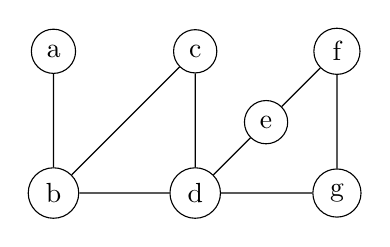
\begin{tikzpicture}
		[scale=1.8,every node/.style={circle,draw=black}]
		\node (a) at (1,2) {a};
		\node (b) at (1,1)  {b};
		\node (c) at (2,2)  {c};
		\node (d) at (2,1) {d};
		\node (e) at (2.5,1.5)  {e};
		\node (f) at (3,2)  {f};
		\node (g) at (3,1)  {g};

		\foreach \from/\to in {a/b, b/c, c/d, b/d, d/e, d/g, e/f, g/f} \draw (\from) -- (\to);
		% \foreach \from/\to in {n6/n4,n4/n5,n5/n1,n1/n2,n2/n5,n2/n3,n3/n4}
		% \draw (\from) -- (\to);
	\end{tikzpicture}
	\caption{\label{fig:treegraph} Grafen tilhørende træet.}
\end{wrapfigure}

I Figur~\ref{fig:treegraph} ses et eksempel på en graf hvor vertex coveret fundet ved hjælp af træsøgningsalgoritmen bliver $\{b,d,f\}$, og præcis den walk der går ned ad kant $b$, så $d$ og sidst $f$ er den eneste der giver et vertex cover hvis $k = 3$.

\newpage
Størrelsen af træet er højest $k-1$ og dybden er $k$, dermed er der højest $2^{k}-1$ delproblemer. Vi får fra regel 2 i vores kernelisering at hvis $d(v) \ge k+1$ skal den ud, så derfor kan vi antage at $\forall v \in V' \mid d(v) \le k$ og dermed $E = \frac{1}{2} \sum_{v \in V} \le \frac{1}{2}nk$. Dermed kan hver af de $2^{k}$ delproblemer løses i tid $O(nk)$, så den endelige køretid er $O(m+nk \cdot 2^{k})$.

\section{Eksakte Algoritmer}%
\label{sec:exactalgorithms}

\begin{note}[Kilder]
	Video 26
\end{note}

\begin{theorem}
	Hvert problem i $\mathcal{NP}$ kan løses i eksponentiel tid.
\end{theorem}

\begin{proof}
	Lad $L$ være et problem i $\mathcal{NP}$, og lad $p(k)$ være et polynomium, så vi har: $x \in L$ hvis og kun hvis der findes en streng $y = y(x)$ af længde højst $p(|x|)$, så $A(x,y) = 1$, hvor $A = A(L)$ er en verifikator, der tjekker certifikater for $L$.

	Strengen $y(x)$ er en bitstreng med længde højst $p(|x|)$. Ved at teste højst $2^{p(|x|)}$ bitstrenge $w$ for at se, om $A(x,w) = 1$, kan vi afgøre, om $x$ er i $L$ i tid $O(2^{p(|x|)}|x|^c)$ for en konstant $c$.
\end{proof}

Vi definerer ny en ny notation, $O^{*}$ til at være aysmptotisk $O$-notation, men hvor vi ignorerer de polynomielle faktorer. Dermed vil $O(n^{3}\log^{2}n 3^{n/2}) = O^{*}(3^{n/2})$.

\subsection{Optimal Løsning til \textsc{Vertex-Cover}}%
\label{subsec:vcoptimalexact}



Husk træsøgningen for \textsc{Vertex-Cover} problemet i delkapitel~\ref{subsec:treesearch}. Der bruge vi et træ til at finde en dækning af størrelse $k$, men vi kan bruge den samme strategi til at finde den optimale dækning.

\begin{wrapfigure}{r}{0.5\textwidth}
	\centering
	\begin{tikzpicture}[
		level 1/.style={sibling distance=6cm},
		level 2/.style={sibling distance=3cm},
		level 3/.style={sibling distance=1.5cm},
		edge from parent/.style={draw, -{Latex}},
		edge from parent path={(\tikzparentnode) -- (\tikzchildnode)},
		scale=0.6
		]

		% Root
		\node {$\circ$}
		child {node {$\circ$}
				child {node {$\circ$}
						child {node {$\circ$}}
						child {node {$\circ$}}
					}
				child {node {$\circ$}
						child{node {$\circ$}}
						child{node {$\circ$}}
					}
			}
		child {node {$\circ$}
				child {node {$\circ$}
						child{node {$\circ$}}
						child{node {$\circ$}}
					}
				child {node {$\circ$}
						child {node {$\circ$}}
						child {node {$\circ$}}
					}
			};


		% Labels
		\node[right] at (2,-0.5) {$v_1$};
		\node[right] at (4,-2.0) {$v_2$};
		\node[right] at (5,-3.5) {$v_3$};

		% Set X
		\node[below right] at (4.5,-4.5) {$X = \{v_1, v_2, v_3\}$};

		% Initial X
		\node[left] at (-4.5,-5.0) {$X = \emptyset$};

	\end{tikzpicture}
	\caption{\label{fig:treesearchoptimal} Træsøgning til optimal dækning.}
\end{wrapfigure}

Hvert niveau repræsenterer en knude som kan blive en del af dækningen. Hvis man går til højre i træet, vælger man at tage den knude, som niveauet repræsenterer, og går man til venstre tager man den ikke. I Figur~\ref{fig:treesearchoptimal} ses et eksempel på hvor alle knuder tages helt til højre, og hvor ingen knuder tages, helt til venstre. Bemærk at vejen der går til venstre to gange, og så en gang til højre, vil have $X = \{v_{3}\}$.

Vi vil nu forsøge at begrænse antallet af knuder. Lad $G$ have $n$ knuder. Husk at vi kan begrænse arbejdet vi laver ved at kigge på antallet af blade i et binært søgetræ. Hvis det har $\ell$ blade, så løser vi højest $2\ell-1$ delproblemer, som er antallet af knuder i søgetræet. Ved \textsc{Vertex-Cover} har søgetræet en dybde på højest $n = |V(G)|$. I det værste tilfælde skal vi løse alle delproblemerne i bladene.

Lad $T(n)$ være antallet af blade i søgetræet for grafer på $n$ knuder. $T(n) \le T(n-1) + T(n-1)$ og $T(1) = 2$, da der er to blade per knude. Dermed $T(n) \le 2^n$. Dermed får vi en $O^{*}(2^{n})$ algoritme. Det er stort set det samme som bare at prøve alle delmængder, så derfor ikke en god algoritme. Vi har to muligheder for hvordan vi skal gøre denen algoritme bedre:
\begin{enumerate}
	\item Gå deltræet igennem på en klog måde, og brug viden om dækningerne vi har set indtil videre.
	\item Brug problemspecifikke observationer til at reducere antallet af blade i søgetræet.
\end{enumerate}

I forhold til mulighed 1: antag at vi allerede har fundet en dækning af størrelse $r$, så behøver vi ikke bruge mere end $r-1$ accept-skridt (gåen til højre i søgetræet). Altså kan vi blive ved med at søge i resten af træet, så længe antallet af skridt er mindre end $r$.

En anden ting at tænke på, er hvordan vi skal gennemgå træet. Ved \textsc{Breadth-First-Search} (BFS) går vi alle knuderne igennem på hvert niveau, før vi går endnu et niveau ned. Dette kræver at vi gemmer på alle delproblemerne, før vi løser dem, hvilket kræver meget hukommelse. Til at gå søgetræet igennem bruger vi en teknik der hedder \textit{Branch and Bound}. Det forklares ikke hvordan den fungerer.

I forhold til mulighed 2: Da vi brugte reduktionsregler i FPT algoritmen til \textsc{Vertex-Cover}, så vi at vi kunne reducere en instans hvor alle knuder har en grad på mindst 2. Dermed, når vi gennemgår søgetræet og vælger ikke at tage en knude med, skal vi inkludere mindst to knuder i den dækning vi bygger til det deltræ, da vi kommer til at mangle de to naboer, som knuden ville have dækket. Derfor kan vi lave følgende grænse:
\begin{equation*}
	T(n) \le T(n-1) + T(n-3), T(1) = 2
\end{equation*}

Løsningen er $T(n) \le 1.4656^{n}$ hvilket betyder at vi kan løse dækningen i tid $O^{*}(1.4656^{n})$.

\begin{lemma}
	\label{lemma:2knudern2}
	Vi kan finde en minimumsdækning i en graf $H$ på $n$ knuder, hvor ingen knude har grad større end $2$ i tid $O(n^{2})$.
\end{lemma}

Vi kan dermed antage at der eksisterer mindst én knuder hvis grad er større end eller lig med 3. Dermed kan vi sige, at hvis vi afviser $v$, skal vi inkluderer mindst 3 knuder i det dækningen for det deltræ. Dermed får vi grænsen:
\begin{equation*}
	T(n) \le T(n-1) + T(n-4)
\end{equation*}
Hvilket giver $T(n) \le 1.3803^{n}$. Dermed kan vi løse \textsc{Vertex-Cover} i tid $O^{*}(1.3803^{n})$.

Tilbage til \textsc{Vertex-Cover} med et parameter $k$, altså ikke opmtimalt, så får vi en ny idé: Vi vil kun kigge på knuder i ent kant $(u,v)$, hvor $\max\{d(u), d(v)\} \ge 3$. Hvis $\{\forall u,v : \max\{d(u),d(v)\} \ge 3\} = \emptyset$, så brug Lemma~\ref{lemma:2knudern2}. Ellers så gør som følger. Hvis du ikke inkluderer $u$, hvor $d(u) \ge 3$, så inkludér i stedet alle dens naboer, hvilke der er 3 eller flere af. Da vi kun går til dybde $k$, så kan vi bruge den samme rekursionsligning fra tidligere og få svar på $O^{*}(1.3803^{k})$ tid.

\subsection{Løsning af \textsc{Traveling-Salesman-Problem} ved brug af Dynamisk Programmering}%
\label{subsec:label}

Givet $n$ knuder, $v_{1}, v_{2}, \ldots, v_{n}$ og deres distancer $d(v_{i}, v_{j}) \; \forall i \ne j$. Vi søger en permutation \(\Pi\) af $\{1,2, \ldots, n\}$ således at ligning \ref{eq:jbjsquare2112} er minimeret.
\begin{equation}
	\label{eq:jbjsquare2112}
	m = d(v_{\Pi(n)}, v_{\Pi(i)}) + \sum_{i=1}^{n-1}  d(v_{\Pi(i)}, v_{\Pi(i+1)})
\end{equation}

Vores idé til at løse problemet er som følger: For hver delmængde $S \subseteq \{v_{2}, v_{3}, \ldots v_{n}\}$ og $v_{i} \in S$, lad $OPT[S, v_{i}]$ være længden af den korteste vej som starter i $v_{1}$ og så besøger alle knuder i $S$ og slutter i $v_{i}$. Bemærk at $v_{1} \notin S$, da vi ikke behøver at tage den med i udregningerne, da vi starter og slutter med den uanset. Dermed, hvis $S = \{v_{2}, \ldots, v_{n}\}$, så kan vi definere $m$ som følger:
\begin{equation*}
	m = \min\{OPT[\{v_{2}, v_{3}, \ldots, v_{n}\}, v_{i}] + d(v_{i}, v_{1}) \mid i \in \{2, 3, \ldots, n\}\}
\end{equation*}

Vi udregner $OPT[\{v_{2}, \ldots, v_{n}\}, v_{i}]$ ved at bruge \textit{dynamisk programmering}.

\begin{lemma}
	\begin{equation*}
		OPT[S, v_{i}] =
		\begin{cases}
			d(v_{1}, v_{i})                                                      & \text{ hvis } S=\{v_{i}\}        \\
			\min\{OPT[S-{v_{i}},v_{k}]+d(v_{k},v_{i}) \mid v_{k} \in S-{v_{i}}\} & \text{ hvis} \{v_{i}\} \subset S
		\end{cases}
	\end{equation*}
\end{lemma}

\begin{proof}
	Hvis $S = v_{i}$ følger det fra definitionen at $OPT[S, v_{i}] = d(v_{1},v_{i})$, så vi antager at $|S| > 1$.

	\textbf{MANGLER: Resten af beviset. Jørgen gør det grafisk. Ca. 24-25 minutter i video 26. Han bruger ikke mere end 2 minutter på det.}
\end{proof}

\begin{algorithm}
	\caption{\label{alg:TSPexact} TSP}
	\begin{algorithmic}[1]
		\REQUIRE $\{v_1, v_2, \ldots, v_n\}, d$
		\FOR{$i \leftarrow 2$ \TO $n$}
		\STATE $\text{OPT}[\{v_1, v_i\}, v_i] \leftarrow d(v_1, v_i)$
		\ENDFOR
		\FOR{$j \leftarrow 2$ \TO $n-1$}
		\FOR{$S \subseteq \{v_1, \ldots, v_n\}$ \; $|S| = j$}
		\FOR{$v_i \in S$}
		\STATE $\text{OPT}[S, v_i] \leftarrow \min_{v_k \in S - \{v_i\}} (\text{OPT}[S - \{v_i\}, v_k] + d(v_k, v_i))$
		\ENDFOR
		\ENDFOR
		\ENDFOR
		\RETURN $\min_{v_i \in \{v_2, v_3, \ldots, v_n\}} (\text{OPT}[\{v_1, v_2, \ldots, v_n\}, v_i] + d(v_i, v_1))$
	\end{algorithmic}
\end{algorithm}

\begin{lemma}
	Algoritme~\ref{alg:TSPexact} udregner en minimumskost \textsc{Traveling-Salesman-Problem} tour ved at udregne $O(n^{2}2^{n})$ korteste veje, gennem OPT udregningen.
\end{lemma}
\begin{proof}
	Antallet af vejlængder udregnet i linje 7 er:
	\begin{equation*}
		\sum_{j=2}^{n-1}  \binom{n-1}{j} \cdot \sum_{i=1}^j (j-1)
	\end{equation*}
	Hvor $j$ i binomialudregningen er størrelse $j$ delmængder af en $n-1$ mængde, og $j$ i andet led kommer fra at der i summationen er $j$ valg for $v_{i}$ og $(j-i)$ valg for $v_{k}$. Vi ved at $\sum_{j=1}^n \binom{n}{j} = 2^{n}$, så vi får:
	\begin{equation*}
		\sum_{j=2}^{n-1} \binom{n-1}{j} \cdot \sum_{i=1}^j (j-1) \le n^{2} \sum_{j=1}^n \binom{n}{j} = n^{2} 2^{n}
	\end{equation*}
\end{proof}

Det betyder altså at vi kan løse \textsc{Traveling-Salesman-Problem} i $O(n^{2}2^{n}) = O^{*}(2^{n})$ tid, hvilket er mindre end den naive algoritme, som løser i $O^{*}((n-1)!)$ tid. Den naive algoritmes køretid er eksponentiel, da vi fra Stirling numbers får $O(n!) \approx O(e^{n \ln n})$.

\subsection{FPT versus XP}%
\label{subsec:label}

\begin{definition}
	Et parameteriseret problem $Q$ med parameter $k$ er \textit{slicewise polynomielt} (XP) hvis det kan løses i $O(f(k) n^{g(k)})$ tid for en funktion $f,g$
\end{definition}

Bemærk her at $Q \in FPT \Rightarrow Q \in XP$, da vi kan lade $g(k)$ være en konstant $c$.

\textsc{Clique} er i $XP$: Givet $(G,k)$, prøv alle $\binom{n}{k}$ delmængder, hvor $n = |V(G)|$. Der er $O(n^{k})$ $k$-delmængder af en $n$-mængde. Så \textsc{Clique} er løseligt i $O(n^{k} \cdot k^{2})$ tid.

Spørgsmålet om \textsc{Clique} $\in XP$ er åbent endnu, trods man mener at svaret er \textit{nej}. Antag at vi kan parameterisere \textsc{$k$-Clique} ved at tjekke alle $O(2^{\Delta})$ delmængder af dens naboer. Dermed, når inputtet har maksimumsgrad $\Delta$, så kan vi kigge efter en k-klikke i $O(n \cdot 2^{\Delta} \cdot \Delta^{2})$ tid. Denne er altså FPT, da den er parameteriseret af maksimumsgrad \(\Delta\).


\subsection{Colouring}%
\label{subsec:label}

Vi har tidligere i en opgave vist at $3$-colouring er et $\textsc{NP}$-komplet problem.

\begin{definition}
	\textsc{$k$-Colouring} er et problem der siger, at givet en konstant $k$, er det muligt at have $k$ delmængder af knuder i en graf, således at der ingen kanter er imellem knuderne i hver delmængde, men der er kanter til de andre delmængder.
\end{definition}

\begin{lemma}
	Undtagen hvis $P = NP$, kan der ikke eksistere en algoritme for at løse \textsc{$k$-Colouring} i $O(f(k)n^{g(k)})$ tid.
\end{lemma}
Dettegælder, da det ville betyde at $3$-colouringville være polynomielt.




%%% Local Variables:
%%% mode: latex
%%% TeX-engine: xetex
%%% TeX-command-extra-options: "-shell-escape"
%%% TeX-master: "main"
%%% End:
